\documentclass[11pt, a4paper]{article}

%----------------------------------------------------------------------------------------
%	1. 基础配置与宏包 (Basic Configuration)
%----------------------------------------------------------------------------------------
\usepackage[fontset=ubuntu]{ctex} % 中文支持 (Overleaf推荐使用XeLaTeX编译器)
\usepackage[margin=1in]{geometry} % 页边距
\usepackage{amsmath, amsthm, amssymb} % 数学公式
\usepackage{mathrsfs} % 花体字
\usepackage{booktabs} % 专业表格
\usepackage{enumitem} % 列表定制
\usepackage{fancyhdr} % 页眉页脚
\usepackage{xcolor}   % 颜色支持
\usepackage[explicit]{titlesec} % 标题格式
\usepackage{setspace} % 行间距
\usepackage{parskip}  % 段落间距

% 绘图支持 (PGFPlots & TikZ)
\usepackage{tikz}
\usepackage{pgfplots}
\usepgfplotslibrary{groupplots} % 允许绘制组图
\pgfplotsset{compat=1.18}
\usetikzlibrary{decorations.markings}

% 设置正文行间距 (1.4倍)
\linespread{1.4}

%----------------------------------------------------------------------------------------
%	2. 配色方案 (Color Scheme: Morandi / Academic)
%----------------------------------------------------------------------------------------
\definecolor{primaryColor}{HTML}{003f5c}   % 主色:深蓝 (标题、强调)
\definecolor{boxBack}{HTML}{f0f5f9}        % 盒子背景:极淡蓝
\definecolor{alertBack}{HTML}{fff2f2}      % 警告背景:极淡红
\definecolor{alertFrame}{HTML}{ff6361}     % 警告边框:珊瑚红
\definecolor{defGreen}{HTML}{2d6a4f}       % 定义绿
\definecolor{defBack}{HTML}{d8f3dc}        % 定义背景:极淡绿

%----------------------------------------------------------------------------------------
%	3. 标题样式定制 (Title Formatting)
%----------------------------------------------------------------------------------------
\usepackage[most]{tcolorbox}

% 一级标题样式 (带背景色块)
\titleformat{name=\section}[block]
  {\normalfont\Large\bfseries\color{primaryColor}}{}{0em}
  {%
    \begin{tcolorbox}[
      enhanced,
      colback=primaryColor!10,
      colframe=primaryColor,
      leftrule=4mm,
      rightrule=0mm, toprule=0mm, bottomrule=0mm,
      arc=0mm,
      boxsep=0pt,
      left=10pt, right=10pt, top=8pt, bottom=8pt, 
      width=\dimexpr\textwidth\relax,
      nobeforeafter,
      valign=center
    ]
      \thesection\hspace{0.75em}#1
    \end{tcolorbox}%
  }

% 目录标题样式 (无编号)
\titleformat{name=\section,numberless}[block]
  {\normalfont\Large\bfseries\color{primaryColor}}{}{0em}{#1}

% 二级标题样式 (带下划线)
\titleformat{\subsection}
  {\normalfont\large\bfseries\color{primaryColor}}
  {\thesubsection}{0.5em}
  {#1}
  [\vspace{-0.3em}\color{primaryColor!30}\hrule height 1pt]

%----------------------------------------------------------------------------------------
%	4. 内容盒子设计 (Custom Boxes)
%----------------------------------------------------------------------------------------

% [理论盒子] 蓝色系:用于模型推导、核心理论
\newtcolorbox{theorybox}[2][]{%
  enhanced, colback=boxBack, colframe=primaryColor, coltitle=white,
  fonttitle=\bfseries\sffamily, title={#2},
  attach boxed title to top left={yshift*=-\tcboxedtitleheight/2, xshift=5mm},
  boxed title style={colback=primaryColor, rounded corners=2pt},
  drop fuzzy shadow, #1
}

% [定义盒子] 绿色系:用于定义、假设、约束条件 (支持跨页)
\newtcolorbox{defbox}[1]{%
  enhanced, breakable, % 允许跨页
  colback=defBack, colframe=defGreen, coltitle=white,
  fonttitle=\bfseries\sffamily, title={#1},
  attach boxed title to top left={yshift*=-\tcboxedtitleheight/2, xshift=5mm},
  boxed title style={colback=defGreen, rounded corners=2pt},
  sharp corners
}

% [结论/警示盒子] 红色系:用于重要结论、批判、注意点
\newtcolorbox{alertbox}[2][]{%
  enhanced, colback=alertBack, colframe=alertFrame, coltitle=white,
  fonttitle=\bfseries\sffamily, title={#2},
  attach boxed title to top left={yshift*=-\tcboxedtitleheight/2, xshift=5mm},
  boxed title style={colback=alertFrame, rounded corners=2pt},
  drop fuzzy shadow, #1
}

%----------------------------------------------------------------------------------------
%	5. 页眉页脚 (Header & Footer)
%----------------------------------------------------------------------------------------
\pagestyle{fancy}
\fancyhf{}
% 请根据具体章节修改此处内容
\fancyhead[L]{\sffamily\color{gray} Course Name / Notes Title} 
\fancyhead[R]{\sffamily\color{gray} Chapter X}
\fancyfoot[C]{\thepage}
\renewcommand{\headrulewidth}{0pt} 

%----------------------------------------------------------------------------------------
%	文档开始 (Document Start)
%----------------------------------------------------------------------------------------
\begin{document}

% --- 封面区域 (Cover Page) ---
\begin{center}
    \vspace*{2cm}
    {\Huge \bfseries \color{primaryColor} Course Name / Subject}\\[0.8cm]
    {\Large \itshape \color{gray} Chapter X: Title Here}\\[2cm] % 修改章节标题
    
    \begin{tcolorbox}[colback=gray!10, colframe=gray!10, width=0.7\textwidth]
        \centering \sffamily 
        Author Name | Semester/Year \\[0.5em] 
        \textcolor{gray!80!black}{\footnotesize 编写于 YYYY 年 X 季学期,仅供学习与交流参考,请勿用于商业用途。} 
    \end{tcolorbox}
\end{center}

\tableofcontents
\newpage

%----------------------------------------------------------------------------------------
%	正文内容 (Main Content)
%----------------------------------------------------------------------------------------

\section{第一节标题 (Section Title)}

这里是正文引言。可以使用列表环境:
\begin{itemize}
    \item 关键点 1
    \item 关键点 2
\end{itemize}

\subsection{子标题 (Subsection Title)}

% [使用示例] 定义盒子
\begin{defbox}{定义标题 (Definition)}
\textbf{1. 核心概念:}
这里输入定义的具体内容...
\begin{equation}
    f(x) = \int_0^T e^{-\rho t} u(c_t) dt
\end{equation}

\textbf{2. 补充说明:}
支持列表和跨页显示。
\end{defbox}

\subsection{数学推导示例}

% [使用示例] 理论盒子
\begin{theorybox}{模型/定理名称 (Theory Name)}
这里输入推导过程或核心理论...
\begin{equation}
    H = v(x, c, t) + \lambda g(x, c, t)
\end{equation}
\end{theorybox}

% [使用示例] 警示盒子
\begin{alertbox}{重要结论 (Conclusion)}
这里输入最终的结论或需要特别注意的反直觉结果。
\end{alertbox}

\newpage

\section{绘图模板 (Plotting Templates)}

以下是预设好的绘图模板,复制后修改参数即可使用。

\subsection{模板 1: 左右并排函数图 (Side-by-side Plots)}
% 适用于展示两种情况的对比 (如稳定 vs 不稳定)

\begin{center}
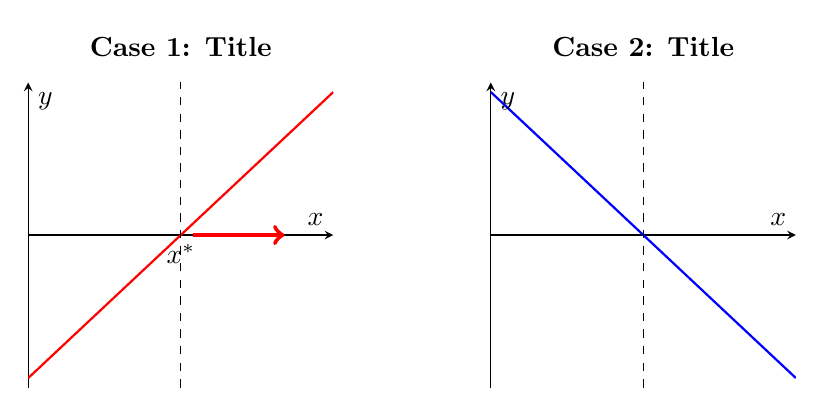
\begin{tikzpicture}
    \begin{groupplot}[
        group style={group size=2 by 1, horizontal sep=2cm},
        width=0.45\textwidth, height=0.45\textwidth,
        axis lines=middle,
        xlabel={$x$}, ylabel={$y$},
        xtick={\empty}, ytick={\empty}, % 不显示刻度
        ymin=-4, ymax=4, xmin=0, xmax=5,
        grid=none
    ]
    % 左图
    \nextgroupplot[title={\textbf{Case 1: Title}}]
        \addplot[thick, red, domain=0:5] {1.5*(x-2.5)}; % 修改函数
        \draw[dashed] (axis cs:2.5, -4) -- (axis cs:2.5, 4); % 辅助线
        \node[below] at (axis cs:2.5, 0) {$x^*$};
        % 箭头示例
        \draw[ultra thick, ->, red] (axis cs:2.7, 0) -- (axis cs:4.2, 0);

    % 右图
    \nextgroupplot[title={\textbf{Case 2: Title}}]
        \addplot[thick, blue, domain=0:5] {-1.5*(x-2.5)}; % 修改函数
        \draw[dashed] (axis cs:2.5, -4) -- (axis cs:2.5, 4);
    \end{groupplot}
\end{tikzpicture}
\end{center}

\subsection{模板 2: 多图并排示意图 (Multiple Phase Diagrams)}
% 适用于展示三种动态特征 (如源、汇、鞍点)
% 纯 TikZ 绘制,不容易报错,修改 scale 可调整大小

\begin{center}
\tikzset{
    arrowstyle/.style={->, >=stealth, very thick, black},
    axisstyle/.style={->, >=stealth, thick, black},
    dotstyle/.style={fill=cyan!50, draw=cyan, thick, circle, minimum size=3pt, inner sep=0pt}
}
\begin{tikzpicture}[scale=0.52] % 缩放以适应一行放三图
    % 图 1
    \begin{scope}[shift={(0,0)}]
        \node[align=center, font=\bfseries] at (0, 5.5) {1. Title};
        \draw[step=1, gray!10, thin, dotted] (-3.5,-3.5) grid (3.5,3.5);
        \draw[axisstyle] (-3.5,0) -- (3.5,0) node[right] {$y_1$};
        \draw[axisstyle] (0,-3.5) -- (0,3.5) node[left] {$y_2$};
        \node[dotstyle] at (0,0) {};
        % 画箭头示例
        \draw[arrowstyle] (1.2,1.2) -- (2.0,1.2); \draw[arrowstyle] (1.2,1.2) -- (1.2,2.0);
    \end{scope}

    % 图 2 (向右平移)
    \begin{scope}[shift={(9,0)}] 
        \node[align=center, font=\bfseries] at (0, 5.5) {2. Title};
        \draw[axisstyle] (-3.5,0) -- (3.5,0);
        \draw[axisstyle] (0,-3.5) -- (0,3.5);
    \end{scope}

    % 图 3 (继续平移)
    \begin{scope}[shift={(18,0)}] 
        \node[align=center, font=\bfseries] at (0, 5.5) {3. Title};
        \draw[axisstyle] (-3.5,0) -- (3.5,0);
        \draw[axisstyle] (0,-3.5) -- (0,3.5);
    \end{scope}
\end{tikzpicture}
\end{center}

\subsection{模板 3: 向量场相图 (Vector Field & Isoclines)}
% 适用于展示复杂的非线性系统或鞍点路径
% 包含:背景向量场 + 等倾线 + 粗箭头示意

\begin{center}
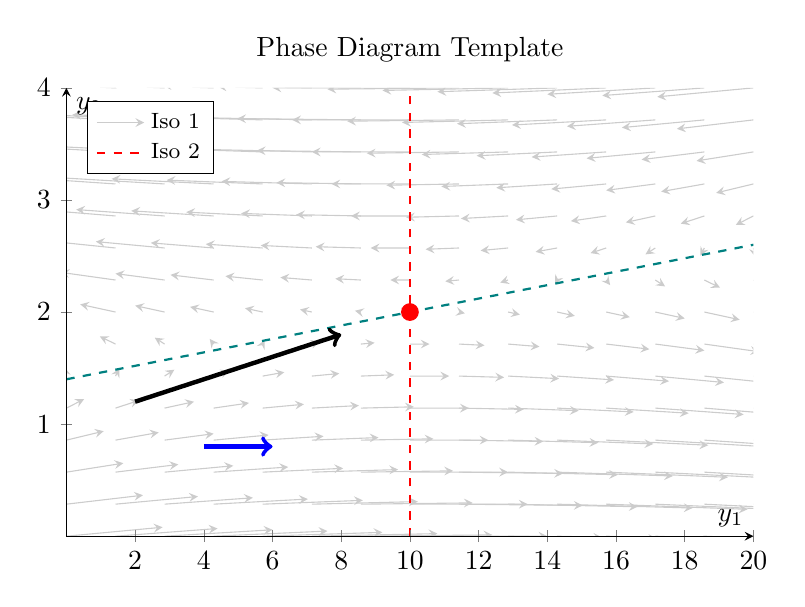
\begin{tikzpicture}
\begin{axis}[
    width=0.85\textwidth, height=0.6\textwidth,
    axis lines=middle,
    xlabel={$y_1$}, ylabel={$y_2$},
    xmin=0, xmax=20, ymin=0, ymax=4,
    grid=both,
    title={Phase Diagram Template},
    view={0}{90}, domain=0:20, y domain=0:4, samples=15,
    legend pos=north west, legend style={font=\footnotesize}
]

% 1. 向量场 (背景)
\addplot3[gray!40, quiver={u={0.06*x - y + 1.4}, v={-0.004*x + 0.04}, scale arrows=2}, -stealth] {0};

% 2. 等倾线 (Isoclines)
\addplot[thick, dashed, red] coordinates {(10, 0) (10, 4)}; \addlegendentry{Iso 1}
\addplot[thick, dashed, teal] {0.06*x + 1.4}; \addlegendentry{Iso 2}

% 3. 稳态点
\addplot[mark=*, mark size=3pt, red] coordinates {(10, 2)};

% 4. 示意箭头 (自定义位置)
\draw[->, ultra thick, blue] (axis cs: 4, 0.8) -- (axis cs: 6, 0.8);

% 5. 路径示意
\draw[ultra thick, ->, black] (axis cs: 2, 1.2) -- (axis cs: 8, 1.8);

\end{axis}
\end{tikzpicture}
\end{center}

\end{document}